\let\negmedspace\undefined
\let\negthickspace\undefined
\documentclass[journal]{IEEEtran}
\usepackage[a5paper, margin=10mm, onecolumn]{geometry}
%\usepackage{lmodern} % Ensure lmodern is loaded for pdflatex
\usepackage{tfrupee} % Include tfrupee package

\setlength{\headheight}{1cm} % Set the height of the header box
\setlength{\headsep}{0mm}     % Set the distance between the header box and the top of the text

\usepackage{gvv-book}
\usepackage{gvv}
\usepackage{cite}
\usepackage{amsmath,amssymb,amsfonts,amsthm}
\usepackage{algorithmic}
\usepackage{graphicx}
\usepackage{textcomp}
\usepackage{xcolor}
\usepackage{txfonts}
\usepackage{listings}
\usepackage{enumitem}
\usepackage{mathtools}
\usepackage{gensymb}
\usepackage{comment}
\usepackage[breaklinks=true]{hyperref}
\usepackage{tkz-euclide} 
\usepackage{listings}
% \usepackage{gvv}                                        
\def\inputGnumericTable{}                                 
\usepackage[latin1]{inputenc}                                
\usepackage{color}                                            
\usepackage{array}                                            
\usepackage{longtable}                                       
\usepackage{calc}                                             
\usepackage{multirow}                                         
\usepackage{hhline}                                           
\usepackage{ifthen}                                           
\usepackage{lscape}
\usepackage{circuitikz}


\begin{document}

\bibliographystyle{IEEEtran}
\vspace{3cm}

\title{3.3.7}
\author{AI25BTECH11023-Pratik R}
 \maketitle
% \newpage
% \bigskip
{\let\newpage\relax\maketitle}

\renewcommand{\thefigure}{\theenumi}
\renewcommand{\thetable}{\theenumi}
\setlength{\intextsep}{10pt} % Space between text and floats


\numberwithin{equation}{enumi}
\numberwithin{figure}{enumi}
\renewcommand{\thetable}{\theenumi}

\textbf{Question}:

Write the steps of construction for drawing a $\Delta ABC$ in which $BC= 8cm$, $\angle B= 45$
and $\angle C= 30\degree$

\textbf{solution}:

Let $\myvec{0\\0}$ be the position vector of point $\vec{B}$ and a,b and c be the sides opposite the vertices A,B and C, respectively in $\Delta ABC$.

Given a =8cm;
\begin{align}
    \vec{C}=\myvec{8\\0}
\end{align}
\begin{align}
    \therefore \vec{A}=\myvec{c \cos \angle B\\c \sin \angle B}= \myvec{c\times 1/\sqrt{2}\\c\times 1/\sqrt{2}}
\end{align}
in $\Delta ABC$
\begin{align}
   b \cos \angle C + c \cos \angle B = 8
\end{align}
\begin{align}
    b \sin \angle C - c \sin \angle B = 0
\end{align}
Solving linear Equation in b and c:
\begin{align}
    \myvec{\cos \angle C && \cos \angle B \\
    \sin \angle C && -\sin \angle B} \myvec{b \\ c} = \myvec{a\\0}
\end{align}
using augmented matrix
\begin{align}
     \myvec{\cos \angle C & \cos \angle B &\vrule &a \\
    \sin \angle C & -\sin \angle B &\vrule &0} \\
\end{align}
putting $\angle C = 30\degree$ and $\angle B = 45\degree$
\begin{align}
    \myvec{\sqrt{3}/2 & 1/\sqrt{2} &\vrule &8 \\
    1/2 & -1/\sqrt{2} &\vrule &0}
\end{align}
Echelon form of the matrix is given by 
\begin{align}
    \myvec{\sqrt{3}/2 & 1/\sqrt{2} &\vrule &8 \\
    0 & (-\sqrt{3}-1)/\sqrt{2} &\vrule &-8}
\end{align}
\begin{align}
    \frac{(-\sqrt{3}-1)}{\sqrt{2}} \times c = -8
    \end{align}
    \begin{align}
        \implies c = \frac{8\sqrt{2}}{(\sqrt{3}+1)} = \sqrt{3}-1
    \end{align}
    \begin{align}
        \therefore \vec{A}=\myvec{\sqrt{3}-1 \\ 
        \sqrt{3}-1}
    \end{align}
  
\begin{figure}[H]
    \centering
    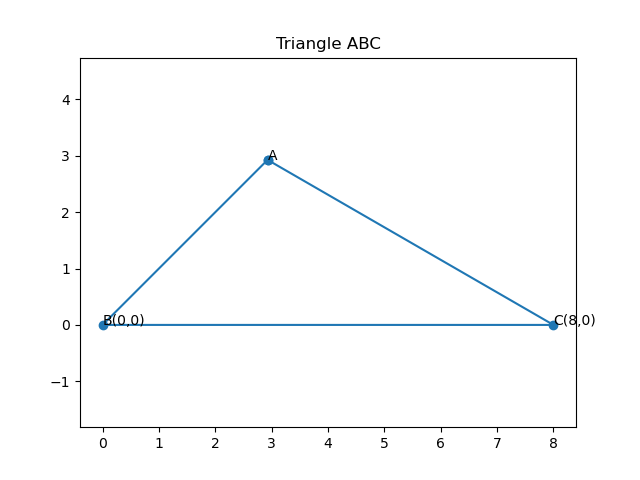
\includegraphics[width=0.8\columnwidth]{figs/fig.png}   
    \label{fig-1}
\end{figure}

 


\end{document}